%%=============================================================================
%% Methodologie
%%=============================================================================

\lstset{
	basicstyle=\ttfamily,
	columns=fullflexible,
	frame=single,
	breaklines=true
}

\chapter{\IfLanguageName{dutch}{Proof of Concept}{Proof of Concept}}
\label{ch:proofofconcept}

\section{Setting up a new Drupal 9 site}

Creating a new Drupal 9 site with the standard Drupal 9 profile on a local server environment is fairly simple. Some different steps are involved depending on the Operating System, but overall the workflow goes like this: 
\begin{itemize}
	\item Create a local environment using an AMP (Apache HTTP server, MySQL relational database, PHP programming language) stack. On the most popular OSs, Linux, Windows and MacOS, packages are available that include all of these technologies. These allow for a smooth and simple process of installing a local environment.
	\item Installing Drupal. The latest release of Drupal can always be found on the \url{https://drupal.org} site.
\end{itemize}

\subsection{Setting up a local environment}

In this proof of concept, MAMP was used to set up a local server environment. MAMP is a tool for MacOS that allows you to easily set up such an environment. The most important directory within MAMP is the htdocs directory. This folder houses all the Drupal files. 

\begin{figure}
	\centering
	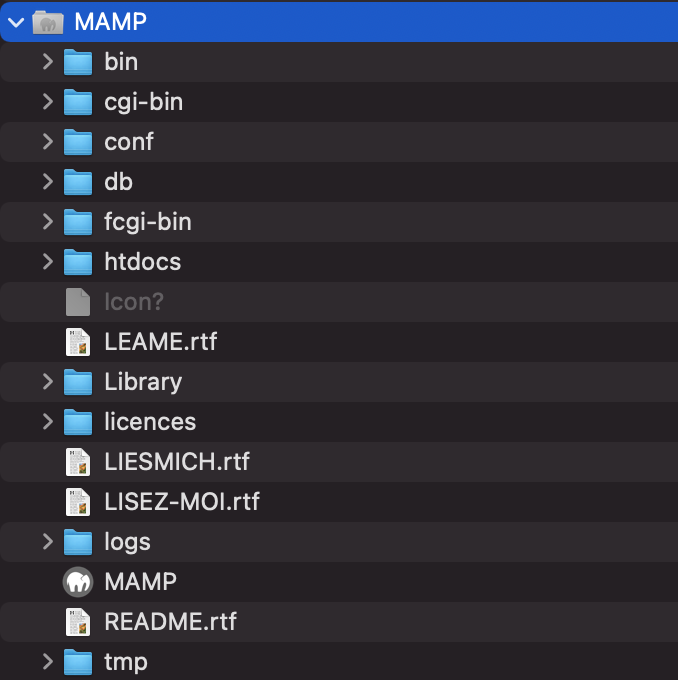
\includegraphics[width=10cm]{./img/MAMP_Structure.png}
	\caption[MAMP folder structure]{The folder structure provided by MAMP}
	\label{fig:MAMP_Structure}
\end{figure}

The files for Drupal 9 were found and downloaded on \url{https://drupal.org/download}. They were then put into the \emph{htdocs} folder inside of MAMP. When starting up MAMP, a graphical interface was launched inside the browser, which had the option to go to your website on the following local address: http://localhost:8888. After that, the actual installation of Drupal could begin.

\subsection{Drupal 9 installation}

Drupal 9 can be installed in two ways: by using drush, or by using the graphical user interface. 

Drush is, according to \textcite{Tomlinson2015}, \emph{"a command line tool that greatly simplifies the tasks of building and administering a Drupal website."} Drush allows you to perform specific tasks related to your Drupal website, one of which is installing the website.

For this proof of concept, the Drupal 9 graphical user interface was used, as it is still the most straight forward way of installing Drupal. When using this interface, Drupal 9 will prompt you through a few steps:

\begin{enumerate}
	\item Choosing the default installation language. English was used here.
	\item Choosing an installation profile. Drupal 9 core comes with two default profiles that can be chosen. Firstly there is the standard profile. This profile comes with commonly used features already pre-configured. Secondly, the minimal profile is used to build a completely custom site without pre-configured functionality. There is also a demo profile included, which comes with some content already in the system. This can be used for testing out the possibilities of Drupal 9. The standard profile was chosen, as it provides some important features that would be used.
	\item Setting up the database. In this case, and in most other cases, this step was configured automatically by the installer. on some rare occasions though, there might be an issue that needs to be resolved by the site administrator. 
	\item Install site. This step automatically installed the Drupal 9 site on the local environment. As with the previous step, there might be some issues that need to be resolved before the installation can be completed.
	\item Configuration of the site. In this step, some important settings needed to be configured. The site information, including the site name and e-mail address, needed to be filled in, and an administration account needed to be configured for this website. As it is a best practice, this account was named \emph{admin}. After that, regional settings and update information needed to be configured. Belgium was chosen as default country, and the default time zone was set to be Brussels.
	\begin{figure}
		\centering
		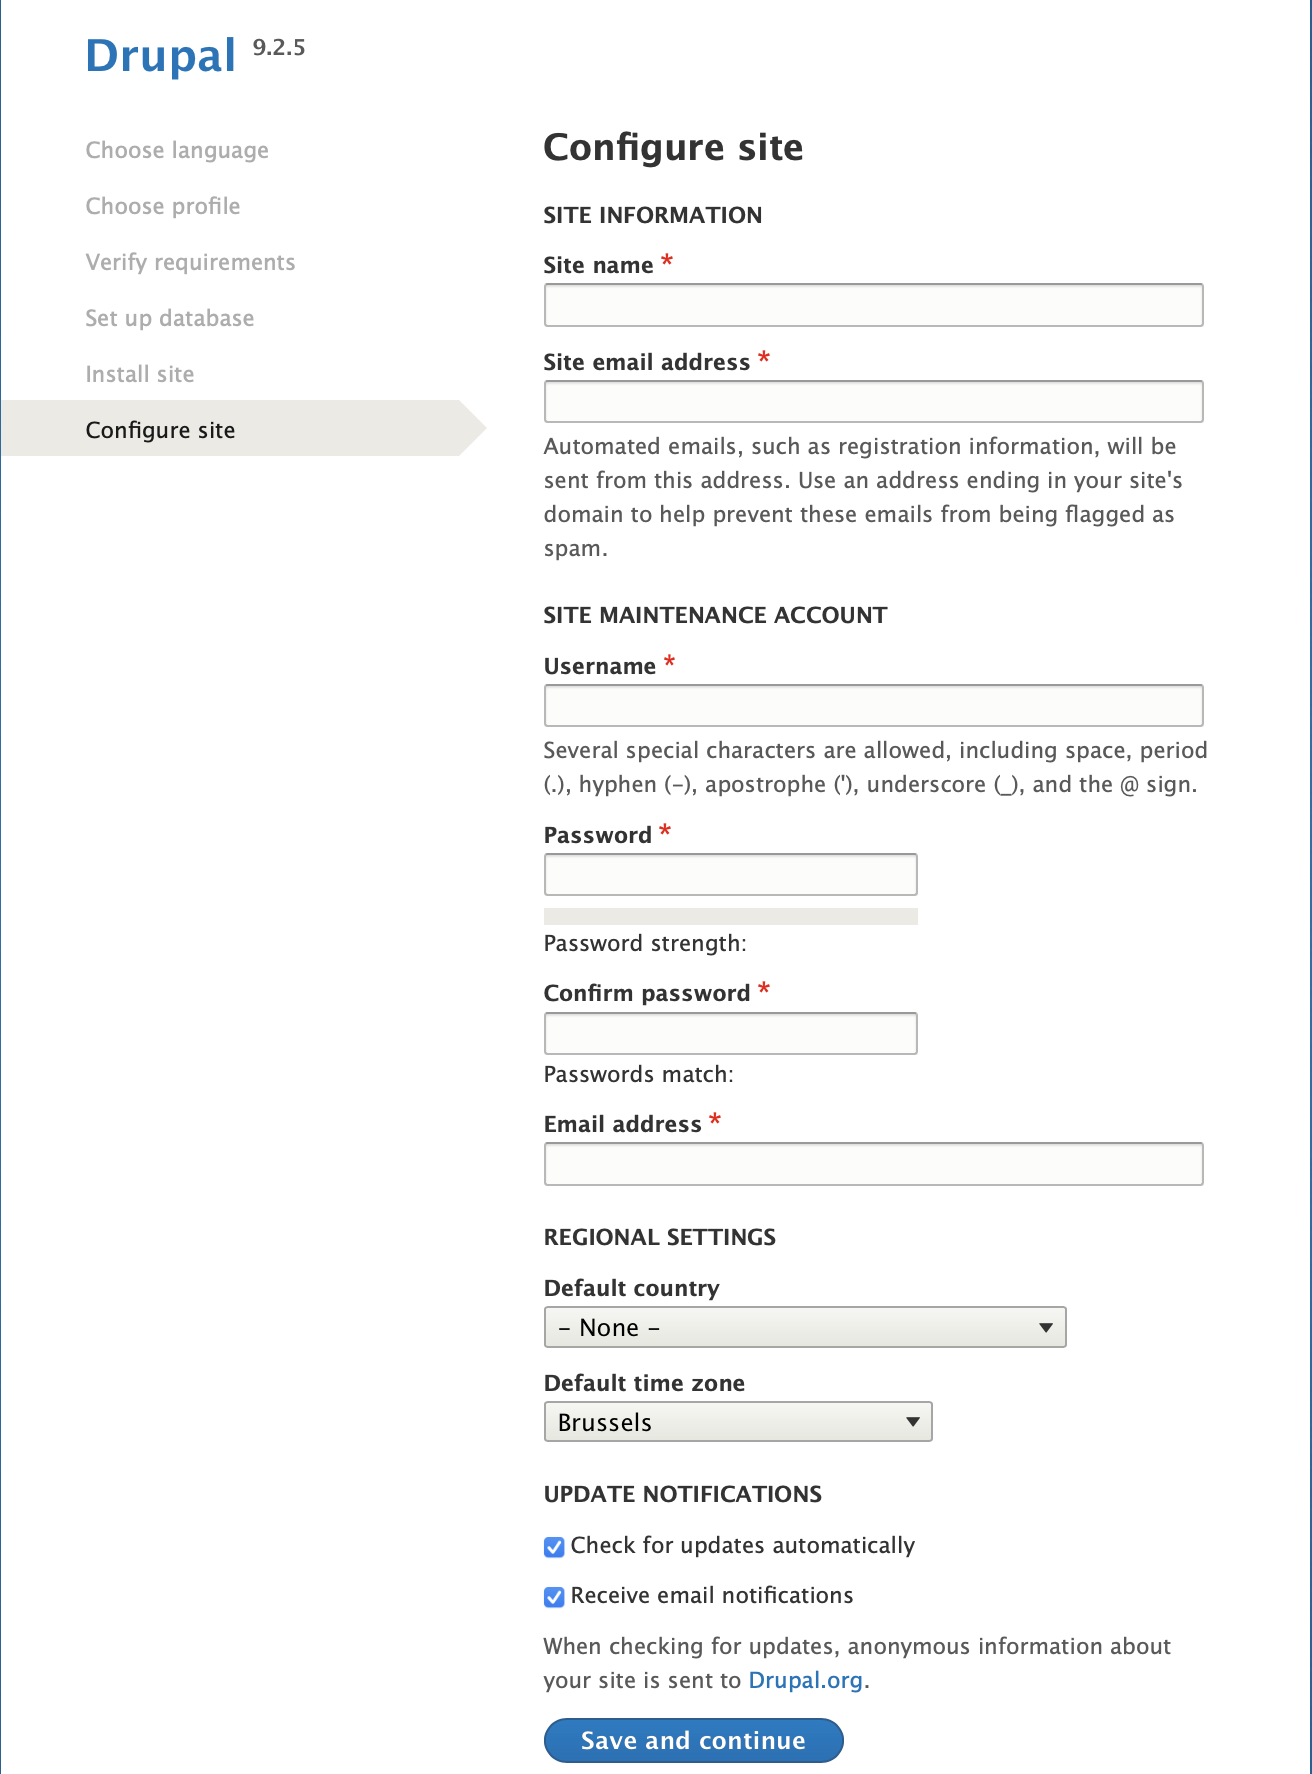
\includegraphics[width=10cm]{./img/Install_Config.png}
		\caption[Configuring Drupal 9]{Configuring your Drupal 9 site}
	\end{figure}
\end{enumerate}

When all these steps were completed, a new Drupal 9 site was ready for use. Before getting started with adding content to the site, a few optional steps were considered that could improve the user experience of the website.

\subsubsection{Installing modules and themes}

Installing modules in Drupal 9 was a fairly simple process. Modules that are included in Drupal 9 core could be easily enabeled through the user interface by going to \url{http://localhost:8888/admin/modules}. Contributed modules, available on \url{https://www.drupal.org} were a little trickier. The best way to install these was via the use of \emph{Composer}. As mentioned in section \ref{sss:composer} Composer is a dependency manager for PHP.  Using Composer, new modules could be easily installed by running the 'composer require' command in the root of the Drupal project.

One module that was installed that could improve the user experience in Drupal was the \emph{Admin Toolbar} module. The most recent version was installed by using Composer: "composer require 'drupal/admin\_toolbar:3.1'". This module improved the default toolbar by transforming it into a  drop-down. It also has three sub-modules that can be enabled for further customizing the admin toolbar. Only the main module was installed for this proof of concept.

\subsection{Adding content}

New content types could be created by going to \url{http://localhost:8888/admin/structure/types} and selecting the \emph{add new content type} option. This way fields could be configured on those content types.

For the purposes of this proof of concept, to show off the possibilities of headless, two different content types were created that could later be exposed to front-end applications: a \emph{Book} content type and an \emph{Author} content type.

The \emph{Book} content type contains the following fields: 

\begin{itemize}
	\item Title
	\item Abstract
	\item Image
	\item Author (this field will be a reference field referencing the \emph{Author} content type)
\end{itemize}

The \emph{Author} content type contains the following fields:

\begin{itemize}
	\item First Name
	\item Last Name
\end{itemize}

\section{Exposing data}

At the basis of using a headless CMS lies the exposing of data. This means that the data that is available within the CMS is exposed through the use of a file format like JSON or XML, just like it would be done in a traditional web API. When correctly configured, any source can then ask for and receive that data, after which they can do with it as they like. Data can also be sent back to the CMS by client applications. In Drupal 9 there are two main modules that fulfill this purpose: JSON:API and RESTful Web Services. Both of these modules were tested out.

\subsection{The JSON:API module}

The JSON:API module is included in Drupal 9 Core, so there was no need to install it using composer. The module was enabled by going to \url{http://localhost:8888/admin/modules}. When installing this module, the \emph{Serialization} module was automatically installed as well, as it is a dependency for JSON:API.

As explained earlier in section \ref{sss:JSONAPI}, no configuration was needed to make this module work. The only important piece of configuration that exists on this module is the choice to allow all operations (create, read, update and delete) instead of just read operations. By default only read operations are accepted. This configuration was found by going to \url{http://localhost:8888/admin/config/services/jsonapi}. For this case this option was turned on.

From the moment this module was enabled, all of the content available in the system was exposed in a standard, fixed format. This content, in JSON (JavaScript Object Notation) format, could be found at \url{http://localhost:8888/jsonapi/node/{content_type}}, replacing {content_type} with the content type that is needed. The data of the \emph{Book} content type could be found at (\url{http://localhost:8888/jsonapi/node/book}) and looked like this:

\begin{lstlisting}
{
	"jsonapi": {},
	"data": [
	{
		"type": "node--book",
		"id": "4b82e6d3-8138-484d-8c9e-5689ba65a671",
		"links": {},
		"attributes": {
			"drupal_internal__nid": 2,
			"drupal_internal__vid": 2,
			"langcode": "en",
			"revision_timestamp": "2022-05-22T11:42:24+00:00",
			"revision_log": null,
			"status": true,
			"title": "Harry Potter and the Philosopher's Stone",
			"created": "2022-05-22T11:37:07+00:00",
			"changed": "2022-05-22T11:42:24+00:00",
			"promote": true,
			"sticky": false,
			"default_langcode": true,
			"revision_translation_affected": true,
			"path": {},
			"field_abstract": {
				"value": "<p>Harry Potter and the Philosopher's Stone&nbsp;is a&nbsp;fantasy novel&nbsp;written by British author&nbsp;J. K. Rowling. The first novel in ...</p>"
			},
			"field_image": "https://upload.wikimedia.org/wikipedia/en/6/6b/Harry_Potter_and_the_Philosopher%27s_Stone_Book_Cover.jpg"
		},
		"relationships": {
			"node_type": {},
			"revision_uid": {},
			"uid": {},
			"field_author": {
				"data": {
					"type": "node--author",
					"id": "24efb772-0b6f-4ad8-942f-05cf4e725ba9"
				},
				"links": {}
			}
		}
	}
	],
	"links": {}
}
\end{lstlisting}

This is what is called an \emph{end point}. The url of this end point can be used by other applications to get the data that is displayed here. The most important parts of this data are:

\begin{itemize}
	\item \emph{data}: contains all the pieces of content of that specific content type. In this case, this is a list of books.
	\item \emph{type}: shows the content type of this piece of content
	\item \emph{id}: shows the id of this piece of content.
	\item \emph{attributes}: contains all the data of this piece of content. For the book content type, this contains the title and abstract fields of the book. The image field was not available here, as images in Drupal are stored as relationships.
	\item \emph{relationships}: contains the id of any reference fields that might be present on this piece of content. In this case, the id of the author that wrote this book were shown. The image field was also present here.
\end{itemize}

For the authors, a similar end point could be found at \url{http://localhost:8888/jsonapi/node/author}. With any content types there was also the possibility to look up just a single piece of content, instead of showing the entire list. This can be very useful if your site contains a lot of content of a specific type, because having to pull all of these in at once can consume time and resources. Getting a single piece of content could be achieved when the id of the content is known. For example, a single book could be found at \url{http://localhost:8888/jsonapi/node/book/{id}}, with \{id\} being replaced by the id of a specific book.

As you can clearly see, using this module was a very easy way to expose the data of any content types in your system. This was the big upside that was noticed when using this method. The big downside was that there was no apparent way to choose which content was exposed. There was also no way to customize the format of this data, so if you wanted to use the XML format, this would not be possible using this module.


\subsection{The  RESTful Web Services module}

The RESTful Web Services module was another way to expose data on your Drupal 9 site. It was also included in Drupal 9 core, so it just had to be enabled to be used. According to \textcite{So2018} this module gives you the possibility to use HTTP methods like GET, POST and DELETE on content entities (just like the JSON:API module), but also allows you to perform GET requests on configuration entities like vocabularies, user roles or other configuration. As this research mainly handles content, this last option was not used.


To set up this module, some steps were required. Like the JSON:API module, RESTful Web Services also had a dependency on the \emph{Serialization} module. As this module was already enabled when enabling the JSON:API module, it did not have to be enabled again. The \emph{HAL (Hypertext Application Language)} module and the \emph{HTTP Basic Authentication} module were also installed. The big difference when installing this module compared to installing JSON:API was that here content was only exposed per node by default. This meant that a list of content, namely the books, was not exposed by default and would have to be configured later.

To make it easier to expose content with RESTful Web Services, a contributed module called \emph{REST UI} was installed by running "composer require 'drupal/restui:1.20'". The module was then be enabled through the graphical user interface.

As previously mentioned, the list of books that needed to be exposed was not exposed by default with this module. This is where the creation of Views came in. By going to the \emph{Views} tab in the Drupal UI, a new View was be created that would group together the books. With the RESTful Web Services module is enabled, the view configuration page allowed for the creation of a \emph{REST export}. There was an option to define the path to where the books would be exposed, which was chosen to be "/books". 

The data of all books was then exposed to the path provided followed by the type of format. The three formats that could be chosen are JSON, XML. So, to get this data in JSON format, \url{http://localhost:8888/booksrest?_format=json} was used. For XML, this was \url{http://localhost:8888/booksrest?_format=xml}. The configuration of the REST export view is shown in figure \ref{fig:RESTView}. The data for one book in the list, in JSON format, looks like this: 

\begin{lstlisting}
	[
	{
		"nid": [
		{
			"value": 2
		}
		],
		"uuid": [
		{
			"value": "4b82e6d3-8138-484d-8c9e-5689ba65a671"
		}
		],
		"vid": [],
		"langcode": [],
		"type": [
		{
			"target_id": "book",
			"target_type": "node_type",
			"target_uuid": "c002de19-a595-498e-bdd7-b792b28bf7ff"
		}
		],
		"revision_timestamp": [],
		"revision_uid": [],
		"revision_log": [],
		"status": [],
		"uid": [],
		"title": [
		{
			"value": "Harry Potter and the Philosopher's Stone"
		}
		],
		"created": [],
		"changed": [],
		"promote": [],
		"sticky": [],
		"default_langcode": [],
		"revision_translation_affected": [],
		"path": [],
		"field_abstract": [
		{
			"value": "<p>Harry Potter and the Philosopher's Stone&nbsp;is a&nbsp;fantasy novel&nbsp;written by British author&nbsp;J. K. Rowling. The first novel in ...</p>"
		}
		],
		"field_author": [
		{
			"target_id": 1,
			"target_type": "node",
			"target_uuid": "24efb772-0b6f-4ad8-942f-05cf4e725ba9",
			"url": "/node/1"
		}
		],
		"field_image": [
		{
			"target_id": 2,
			"alt": "https://upload.wikimedia.org/wikipedia/en/5/5c/Harry_Potter_and_the_Chamber_of_Secrets.jpg",
			"title": "",
			"width": 255,
			"height": 392,
			"target_type": "file",
			"target_uuid": "467e7908-01b1-4591-9dba-98f3ef1c9dec",
			"url": "http://localhost:8888/sites/default/files/2022-05/Harry_Potter_and_the_Chamber_of_Secrets.jpeg"
		}
		],
	}
	]
\end{lstlisting}

As you can see, this has a fairly similar structure to the one JSON:API offered. What was notable here is the lack of seperation between data and relationships. With RESTful Web Services, any reference field is still treated as a normal field, but contains data that can be used to get the content it is referencing, like the id and the url leading to that node.

\begin{figure}[h]
	\centering
	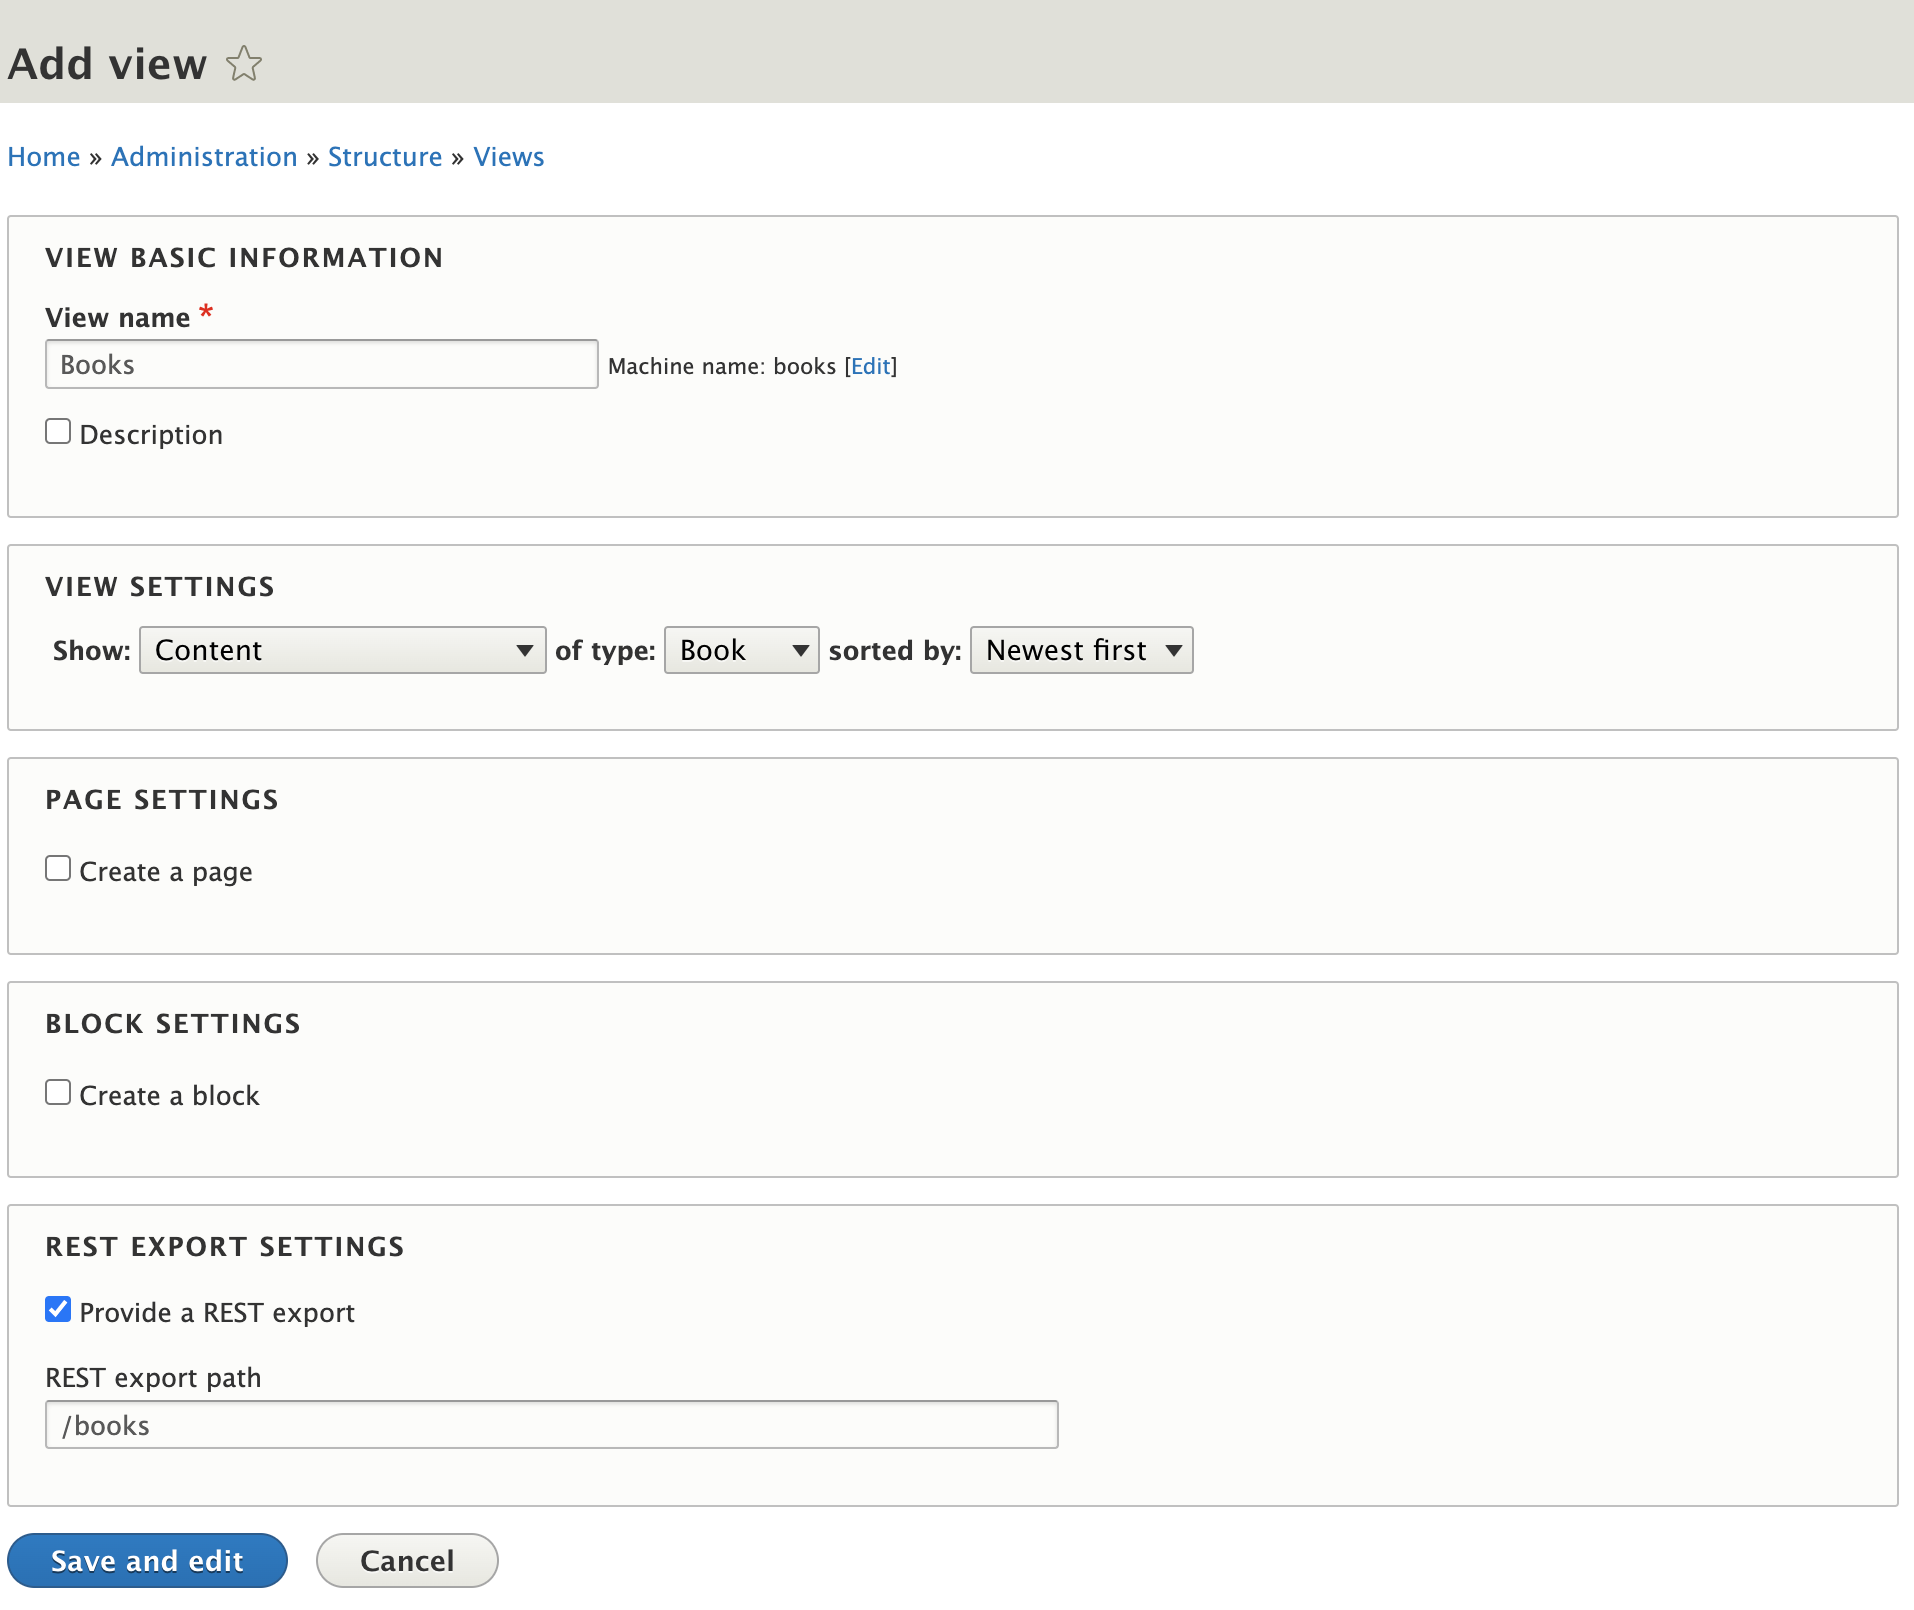
\includegraphics[width=10cm]{./img/View_Create.png}
	\caption[Creating a View]{The configuration page for creating a new view}
\end{figure}

\begin{figure}[h]
	\centering
	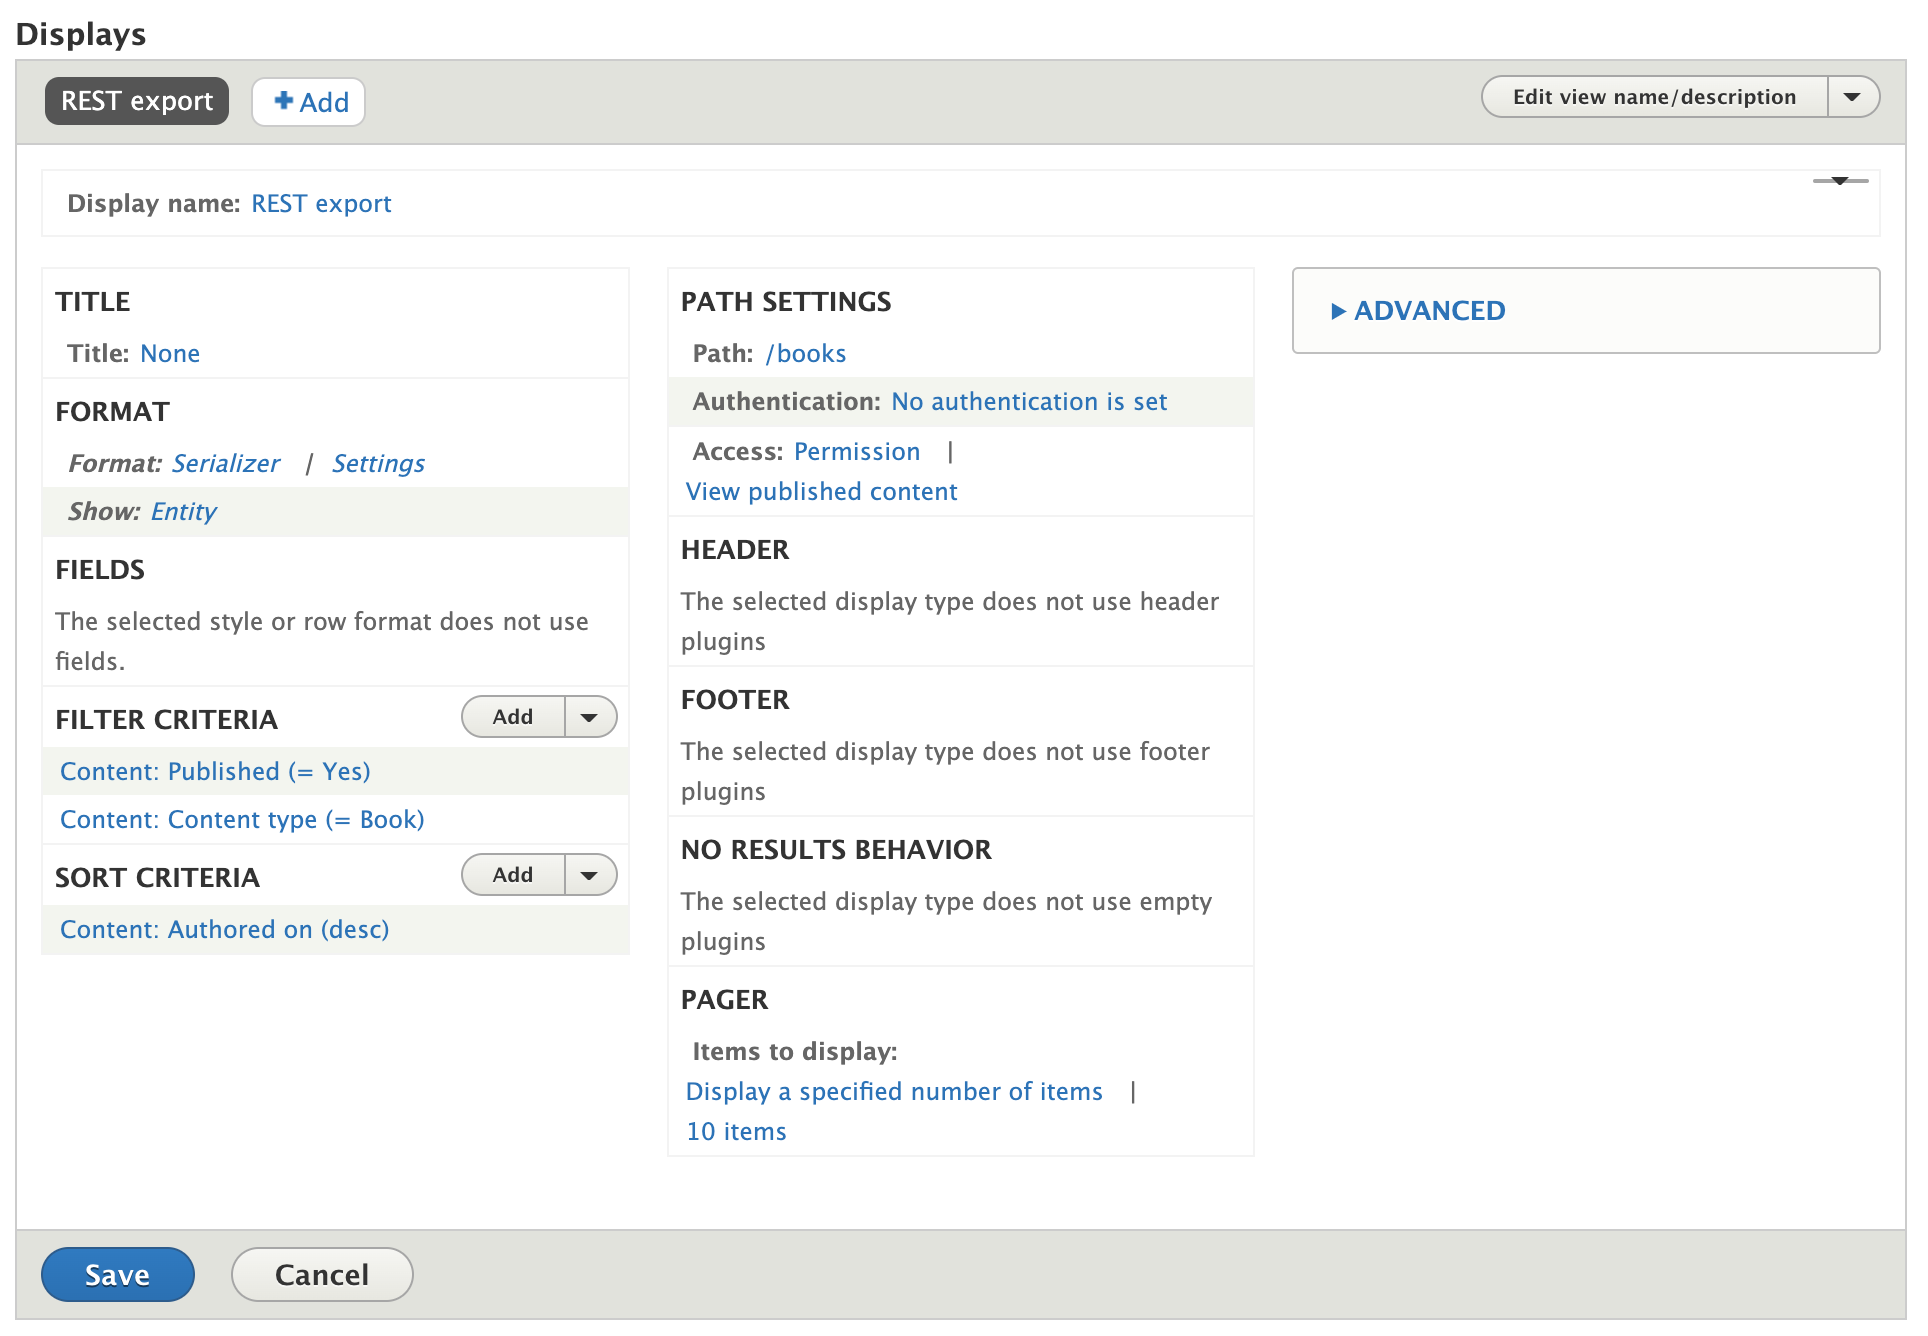
\includegraphics[width=10cm]{./img/View_Details.png}
	\caption[Details of a REST export View]{The details of the REST export view}
	\label{fig:RESTView}
\end{figure}

\subsection{Choosing between JSON:API and RESTful Web Services}

When considering a headless project it is very important to also consider the way to expose data. Both JSON:API and RESTful Web Services are viable options. JSON:API will be more useful for simple projects that don't contain a lot of content. As all of the content gets exposed, websites with a lot of data could suffer a performance hit.

When you want to expose only certain content types, or if you want to expose anything different than a content type, RESTful Web Services will be a better fit. It allows full configuration of which content to expose and in what format. It also gives you the possibility to expose any custom data that might be present in the system.

For the purposes of this proof of concept, the output of the JSON:API module was used to get the data on the front-end, as this is a website with a very small amount of data. The default json format was a natural fit, and no custom data needed to be exposed. 

\section{The front-end}

There are many options to consider on the front-end. These range from the front-end included with Drupal 9, to JavaScript frameworks, to native mobile applications. Basically any framework or tool that has a way to handle HTTP requests through the use of an HTTP client has the possibility to interact with a headless CMS. 

In the following sections the differences between the integrated Drupal front-end and a headless approach will be shown off. Firstly, Drupal Views was used to display a list of the content that was added previously in the back-end. To show off the headless possibilities, the choice was made to use the front-end JavaScript framework Angular. Angular is an extremely popular framework used around the world to create single page applications. It also has a built-in HTTP client that can be used to create any HTTP request and send it to any domain. This way the data in the Drupal back-end was requested and displayed.

\subsection{Drupal 9 front-end}

Displaying the data using Views in Drupal was fairly straight forward. As a view was already created to expose the data using RESTful Web Services, the same view was then used to display the data in Drupal. On the configuration page for the view, a new display was added by choosing the "Add page" button. 

\begin{figure}[h]
	\centering
	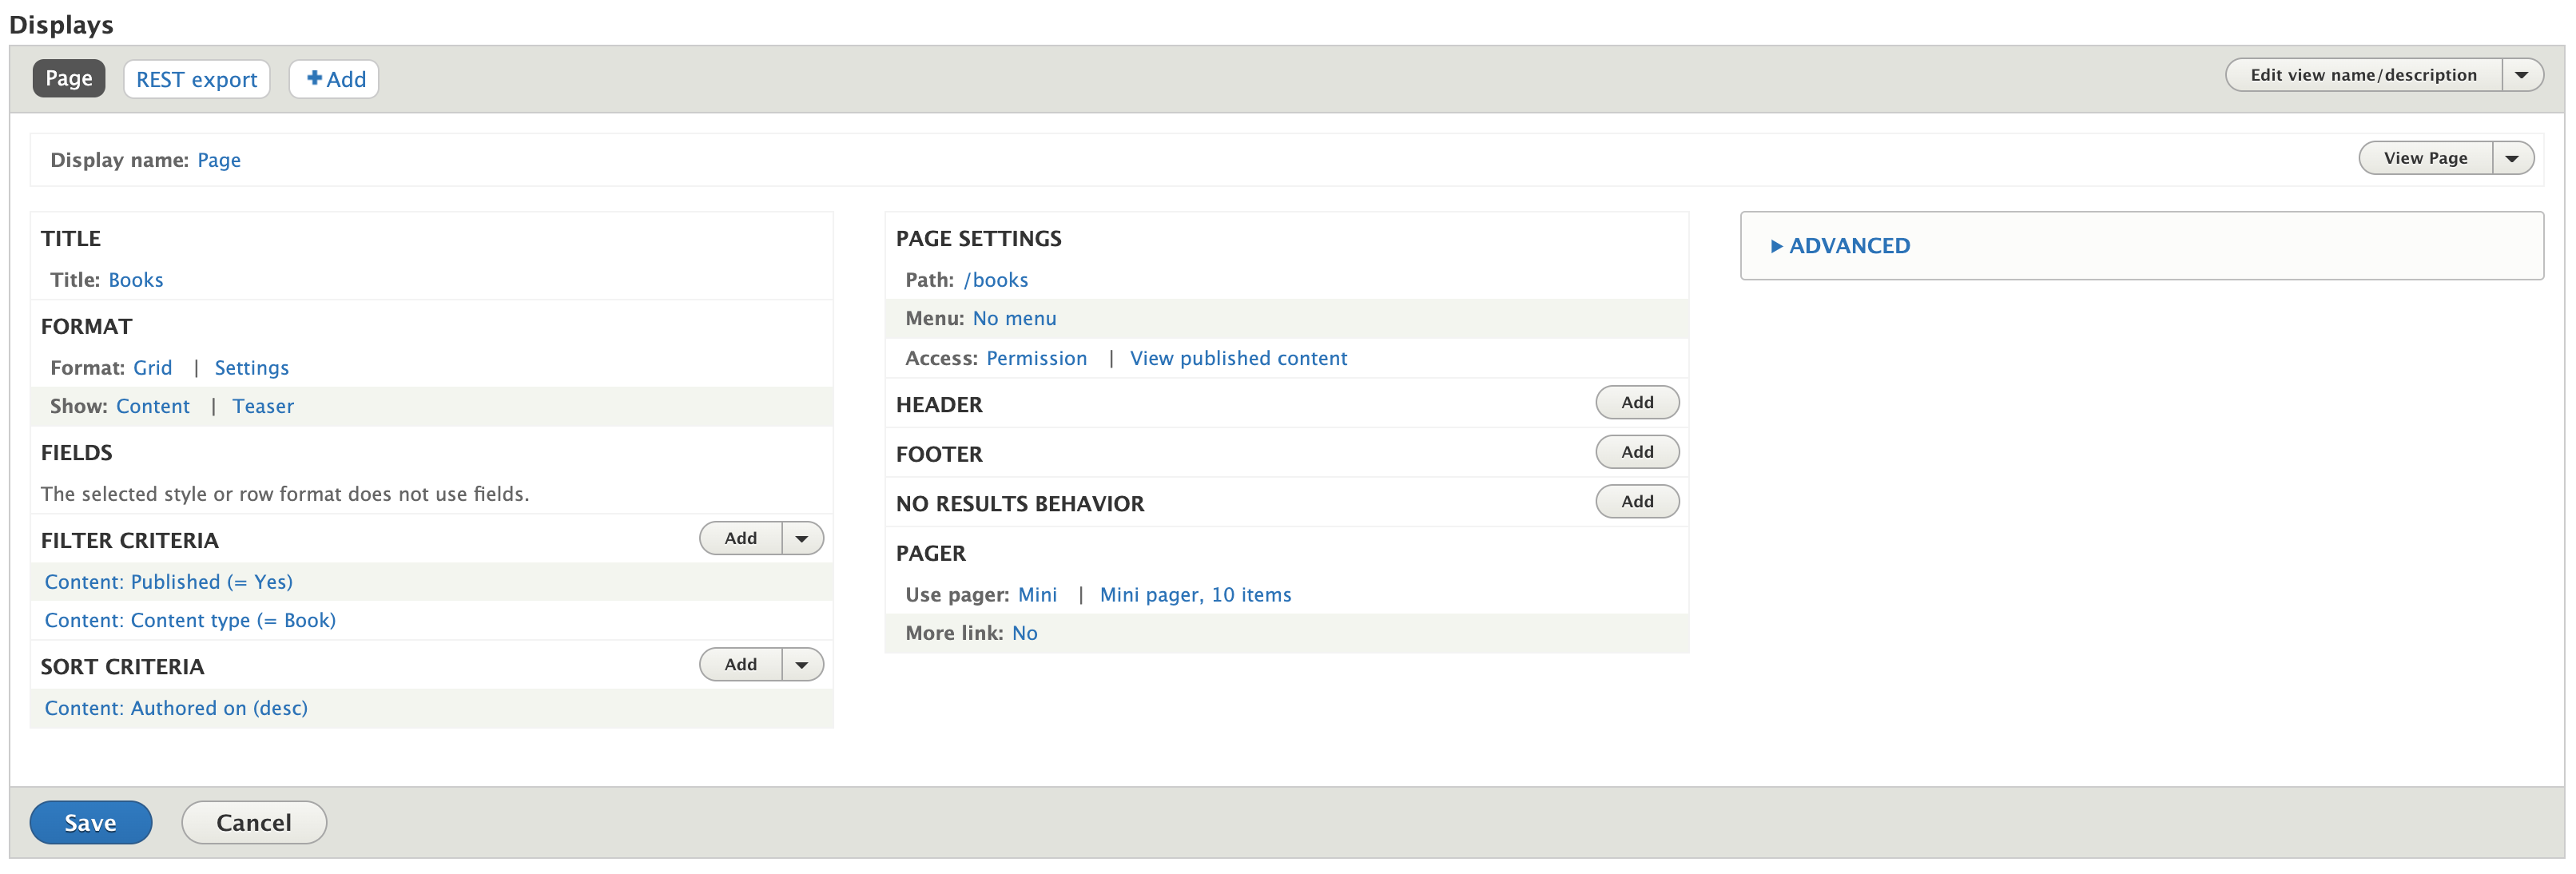
\includegraphics[width=10cm]{./img/Page_View_Config.png}
	\caption[Details of a page display]{The details of a page display}
\end{figure}

This page display was configured so it shows the content in teaser form. In its default form, this just contains the title of the book. To show other fields of this content type, the teaser was configured by going to the content type, and under the "manage display" tab choosing which fields would be displayed for this display. The following fields were added to the display: image, author, and abstract. When these fields were added to this display, the view displayed the list of books like in figure \ref{fig:Books}.

As you can see, this is a pretty quick and easy way to be able to display a list of content. Using views, any content can be displayed this way.

\begin{figure}[h]
	\centering
	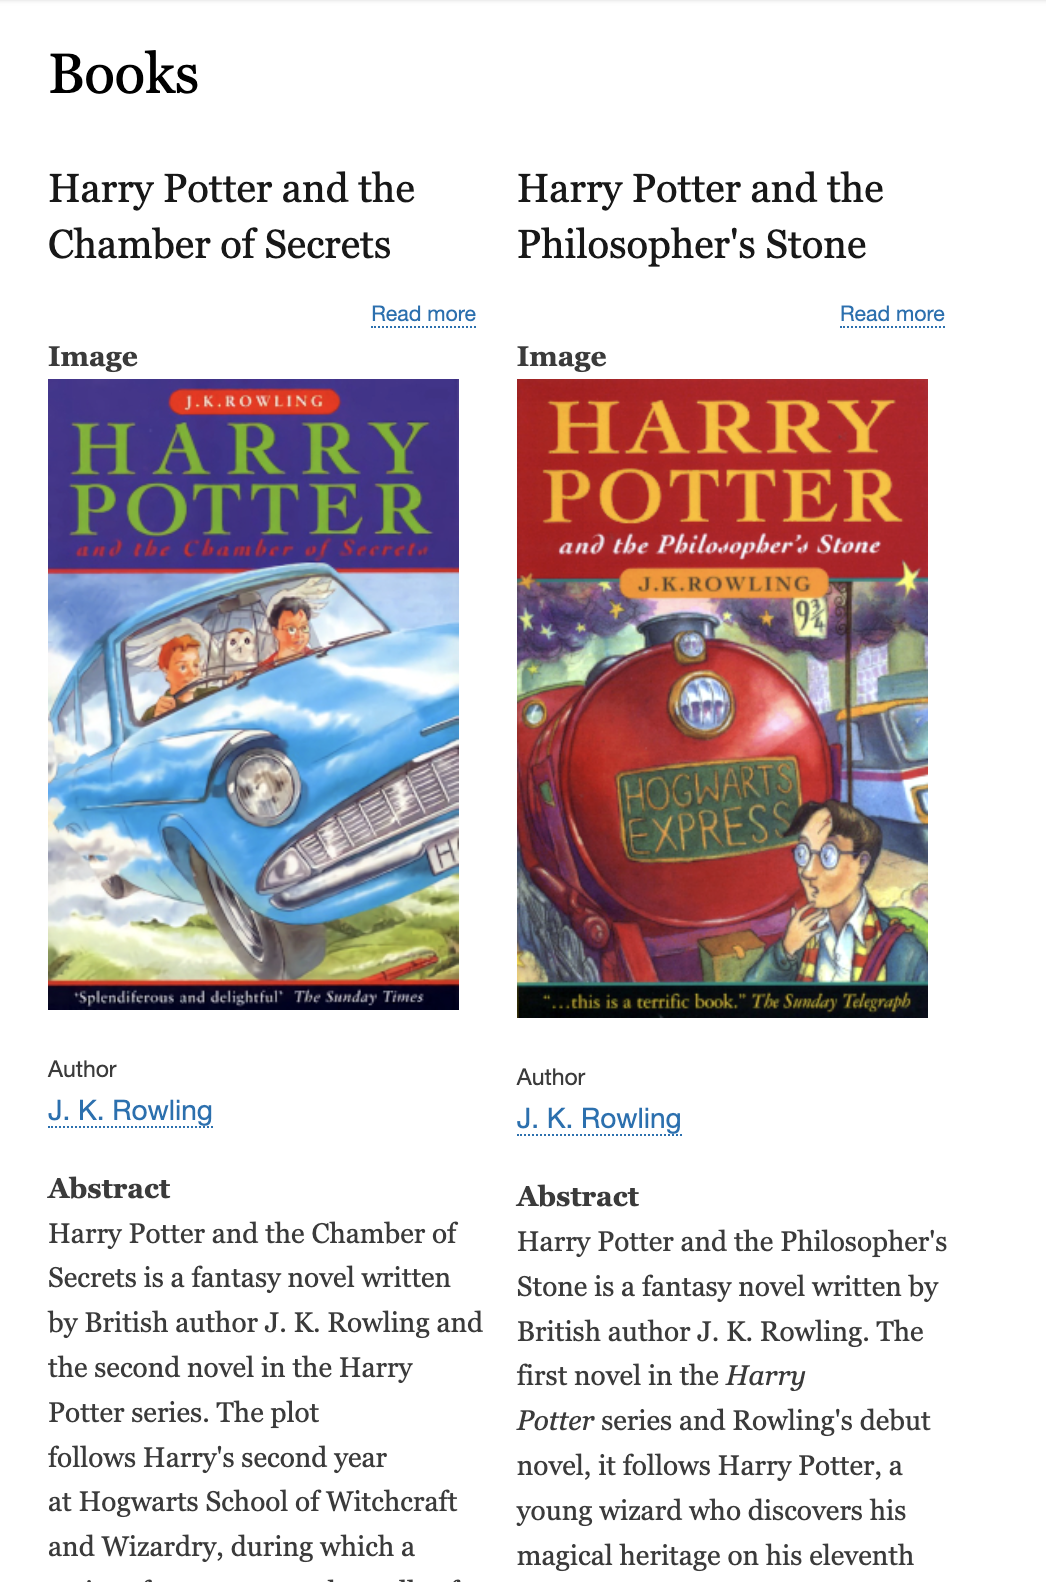
\includegraphics[width=8cm]{./img/Books_Page.png}
	\caption[Display of a list of Books]{The page display of Books displays the fields of all the Books}
	\label{fig:Books}
\end{figure}

\subsection{Single page web application with Angular}

\subsubsection{Preperations and creating a new app}

Creating a new Angular application required a few differerent things. At the foundation of any JavaScript framework lies \gls{Node.js}. Node.js was downloaded and installed from \url{https://nodejs.org/en/}. When installing Node.js, \gls{NPM} was installed with it. With Node.js and NPM installed, the command "npm install --global @angular/cli@9.0.1" was used to globally install the Angular CLI, which would then used to make a new Angular project among other things.

To create a new Angular app, the "ng new {app-name}" command is run, with {app-name} replace by the name of the app. For this case, "ng new headless" is run, which creates an app called "headless". The Angular CLI scaffolds a new Angular app, meaning that it creates all the necessary folders and files to get started with Angular. With the app created, the "ng serve" command is run in the root of the application to start the app.


\subsubsection{Creating a new Angular component}

Creating a new component (or building block) was done by using the Angular CLI. Running "ng new component {component-name}" with {component-name} being replaced by the name of the new component generates all the files needed. For this example "ng generate component book" was run to create a book component. This component displays a single book. 

As another component needed to be created to display the books in a list, module was created by running "ng generate module book --module=app". The "--module=app" option makes sure the module is imported in the app module. This module is used to group together any components related to books.

As the goal is to display a list of books, another component called "Book List" was required. This component was created by running "ng generate component book-list --module=book". This command generated the files for this component and made sure that it is included in the book module.

\subsubsection{Creating a new Angular service}

Services in Angular are used to accomplish specific tasks. One task a service can perform is to make network requests, so a service was needed to get the data from the Drupal back-end. This service was created by running "ng generate service BookService".

To make the connection to the back-end, the Angular HTTP Client was imported from "@angular/common/http". An instance of this HTTP Client was then injected into the service using dependency injection, by including it as an argument in the constructor. This means that whenever this service is created, an HttpClient is passed to it. A get method was then defined to GET all the books from the back-end using the JSON:API URL: \url{http://localhost:8888/jsonapi/node/book/}. The code for this service looks like this: 


\begin{lstlisting}
import { Injectable } from '@angular/core';
import { HttpClient } from '@angular/common/http';
import { Observable } from 'rxjs';
	
@Injectable({
	providedIn: 'root'
})
export class BookService {
		
	constructor(private _http: HttpClient) { }
		
	get books$() : Observable<any>{
		return this._http.get('http://localhost:8888/jsonapi/node/book/');
	}
}
\end{lstlisting}

This method returns all the books from the back-end as an Observable. Any component that wishes to have these books can subscribe to this method. In this case, the book-list component performs this task so it can display the books in a list.

\subsubsection{Subscribing to the service and displaying the data}

To get the data, the book list component subscribes to the method that was defined in the service. The data that is found within the observable was then assigned to a local list that contains books. This all happens within the constructor of the component, so when this component is created it will execute this code and make the call to the Drupal back-end. The code for this component looks like this:

\begin{lstlisting}
	import { Component, OnInit } from '@angular/core';
	import { BookService } from '../book-service.service';

	@Component({
		selector: 'app-book-list',
		templateUrl: './book-list.component.html',
		styleUrls: ['./book-list.component.css']
	})
	export class BookListComponent implements OnInit {
	
		public books: any;
	
		constructor(private _bookService: BookServiceService) {
			_bookService.books$.subscribe(val => this.books = val.data);
		}
	
		ngOnInit(): void {
	}
	
}
\end{lstlisting}

To display the data that is received a few steps were needed. Firstly, some HTML was added in the template for the book-list component. This code uses \emph{ngFor} to loop through the list of books that is kept in this component. It then passes all of those books, one by one, to the book component.
\begin{lstlisting}
<div style="text-align: center;">
	<h1>
		Books:
	</h1>
</div>
<div class="container row">
	<div class="column col-6">
		<div *ngFor="let book of books">
			<app-book [book]="book"></app-book>
		</div>
	</div>
</div>
\end{lstlisting}

Next, the book component needed a field that can contain a single book. This field needed to be annotated with the @Input() decorator, to indicate that this field will be initialized by each book in the book list. Every book in the book list component is passed to the book component this way. As the author of the book is a reference field, the data for that is not immediately available. The easiest way to get this data was by making another request to the back-end using the id of the author (which can be found under the 'field\_author' reference field). This request was made in the ngOnInit() method, so it triggers each time a new book is loaded, meaning that for every book that is loaded on the page a request is sent to receive the author of that specific book.

\begin{lstlisting}
export class BookComponent implements OnInit {
	
	@Input() public book: any;
	public author: any;
	
	constructor(private _bookService: BookService) {
		
	}
	
	ngOnInit(): void {
		if(this.book){
			this._bookService.getAuthor$(this.book.relationships.field_author.data.id).subscribe(val => (this.author = val.data));
		}
	}
	
}

The new method in the book service

export class BookService{
	
	...
	
	getAuthor$(id: string) : Observable<any>{
		return this._http.get(`http://localhost:8888/jsonapi/node/author/${id}`)
	}
	
}
\end{lstlisting}

And finally, some more HTML was added in the template of the book component. This code displays the title, image, and author of the book in a card.

\begin{lstlisting}
	<div class="card" style="cursor: pointer;">
		<div class="card-header">
			<strong>{{book.attributes.title}}</strong>
			<br>
			<img src="{{book.relationships.field_image.data.meta.alt}}" alt="">
			<br>
			<div *ngIf="author">
				{{author.attributes.title}}
			</div>
		</div>
	</div>
\end{lstlisting}

The only thing that needed to be done now is to display the book list component. This was done by adding an "app-book-list" tag in the projects app.component.html file. The following is displayed: 


\begin{figure}[h]
	\centering
	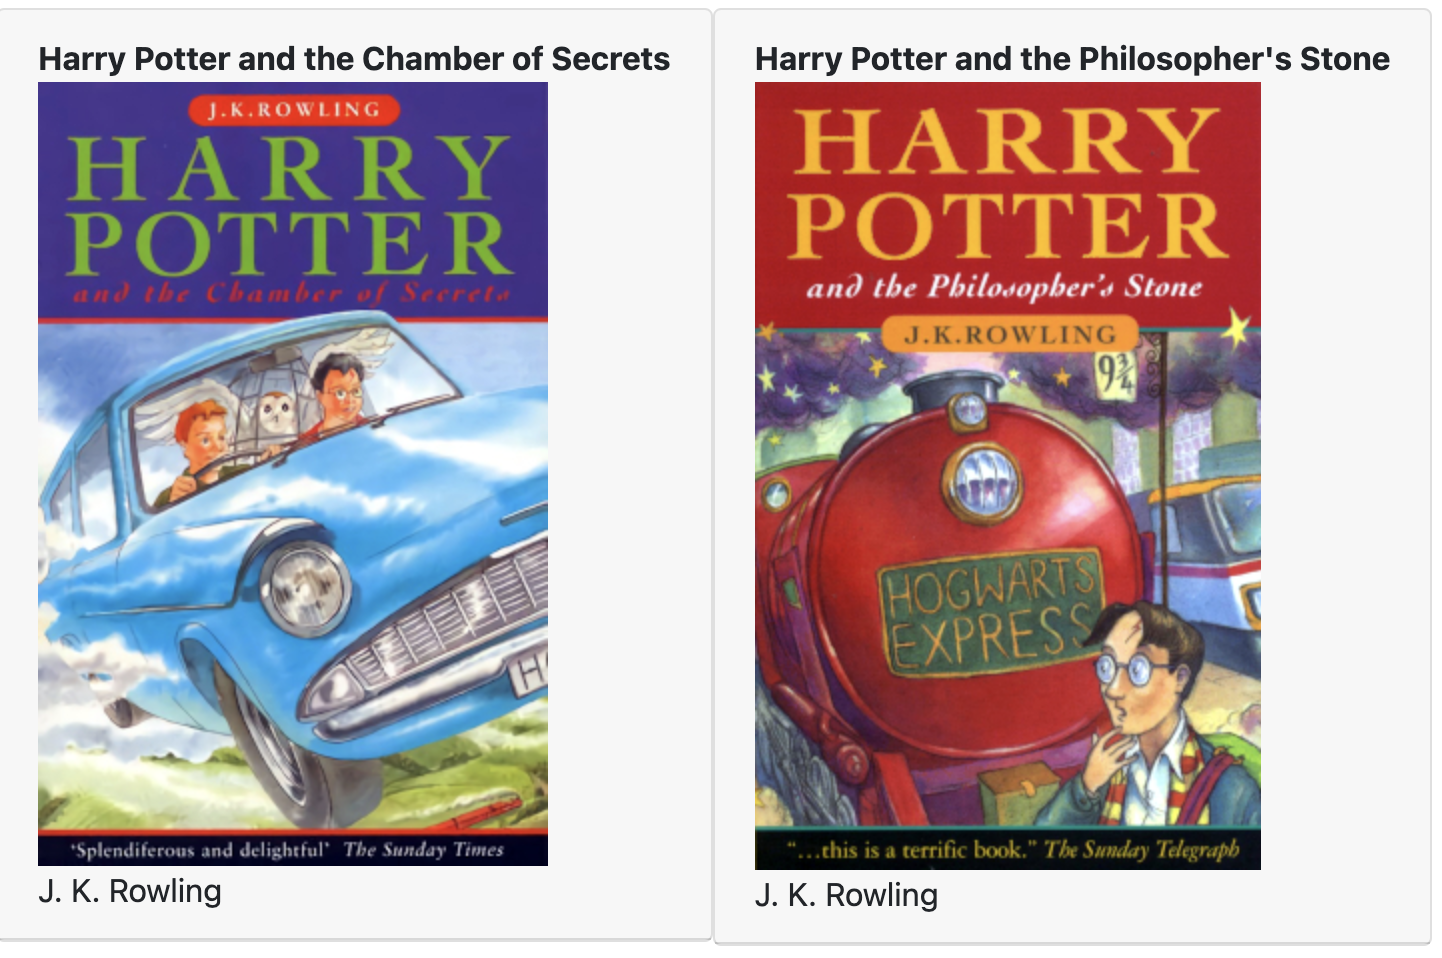
\includegraphics[width=8cm]{./img/Angular_Books.png}
	\caption[Display of a list of Books in Angular]{The overview of Books, displayed in Angular}
	\label{fig:BooksAngular}
\end{figure}

As you can see, this is a very similar result to what was displayed in the Drupal front-end using views.
